\chapter{系统架构}

\section{桌面端架构}

\begin{figure}[H]
  \centering
  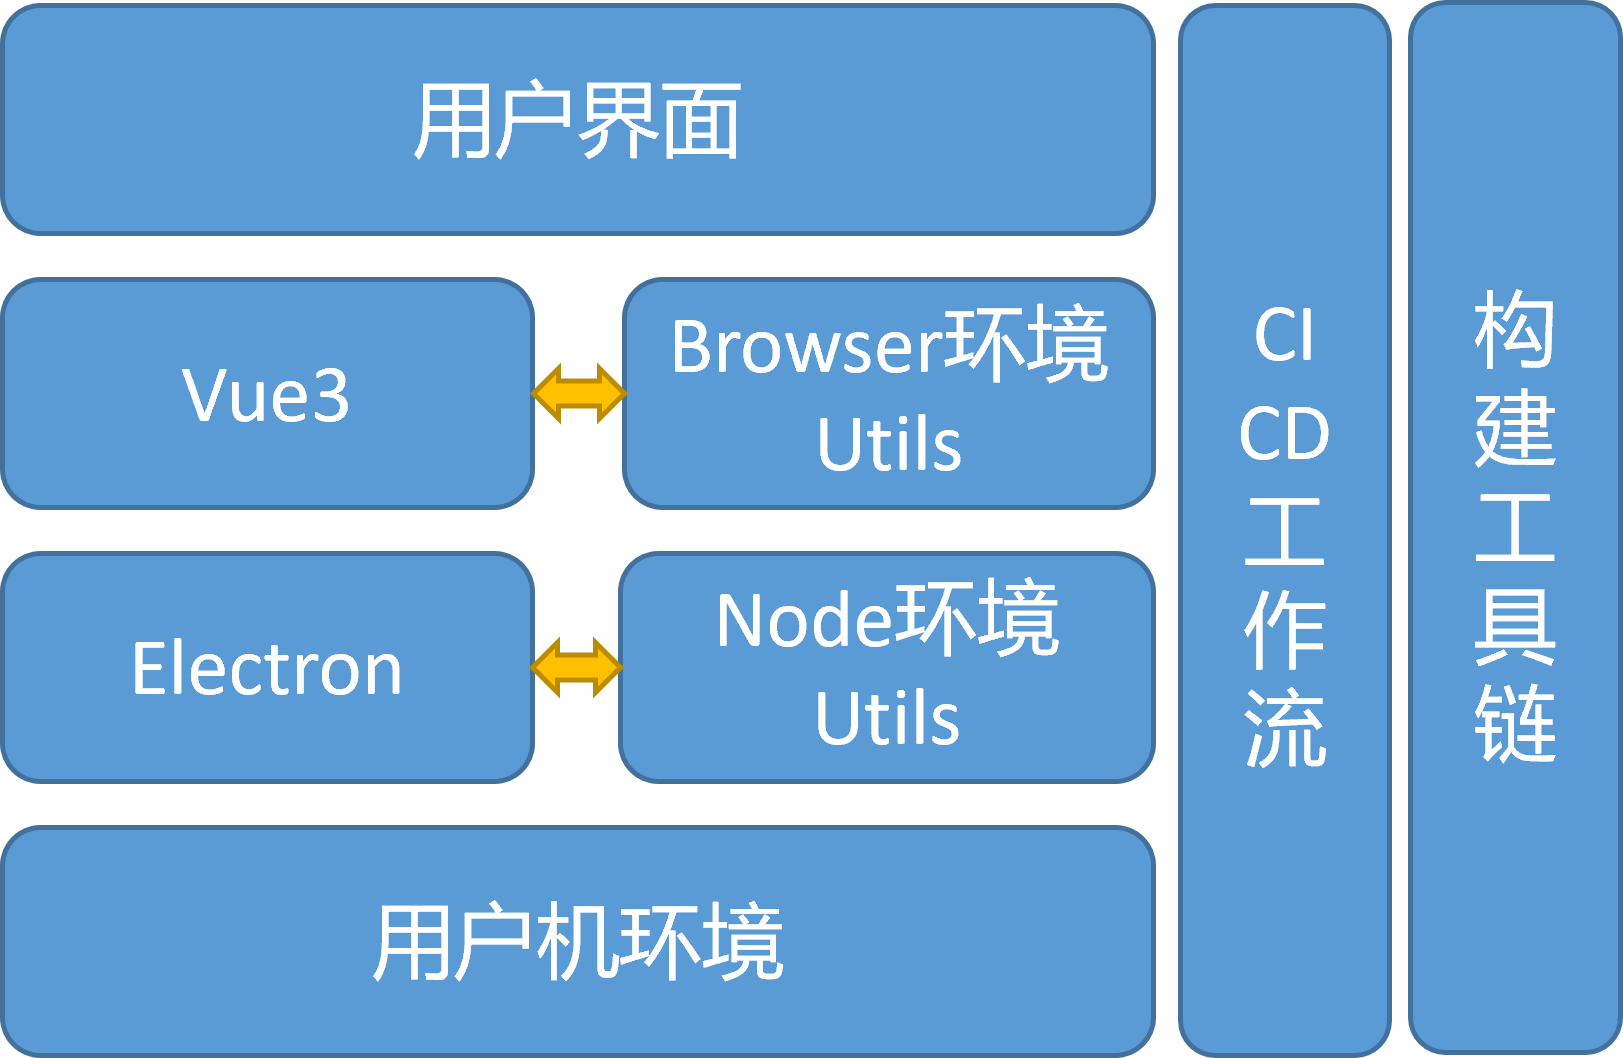
\includegraphics[scale=0.75]{figure/front_arch.png}
  \caption{\textbf{桌面端架构图}}
  \label{fig:front_arch}
\end{figure}

\figref{fig:front_arch}是PhoeniX的桌面端架构图,为了更好地解释该架构图,在此对下文中出现的一些专有名词进行解释:

\begin{enumerate}
  \item Electron:一个用于开发跨平台桌面端应用的框架,包括Visual Studio Code在内的众多软件都使用该框架进行开发,该框架的主要特色在于允许开发者使用Web开发技术开发桌面端应用。
  \item Vite:一个打包与开发Web应用的工具,在本项目中配合Electron-Builder使用,用于将Electron应用打包为应用安装包。
  \item Github Action:将软件开发过程自动化的工具,通常用于软件自动化测试、自动化部署、自动化检查等。
  \item CI/CD:全称为Continuous Integration/Continuous Deployment,即持续集成和持续部署,指软件开发中的一些自动化过程。
  \item Vue3:一个Web前端框架,通常用于网站的开发,可以配合Naive-UI等第三方组件库使用。
  \item Monaco:由微软开发的开源Web编辑器,是微软Visual Studio Code解决方案的一部分,在本项目中配合Vue3使用。
\end{enumerate}

PhoeniX桌面端将TypeScript作为主要的编程语言,相比于JavaScript,TypeScript能够提供更多的类型提示,减少代码编写中的Bug。我们采用Vite和Electron-Builder作为构建工具链,对PhoeniX进行本机调试、应用打包等操作。另外,我们使用Github Action作为核心CI/CD工作流,对PhoeniX进行自动化构建与自动化检查。PhoeniX围绕Electron框架搭建,在Electron框架之上集成了Vue3,使用Electron与用户机进行必要的交互,而使用Vue3完成主要应用逻辑的编写。PhoeniX主要使用Naive-UI构建用户界面,另外还使用了Monaco等第三方组件,提供一致而流畅的用户体验。

\section{服务端架构}

\begin{figure}[H]
  \centering
  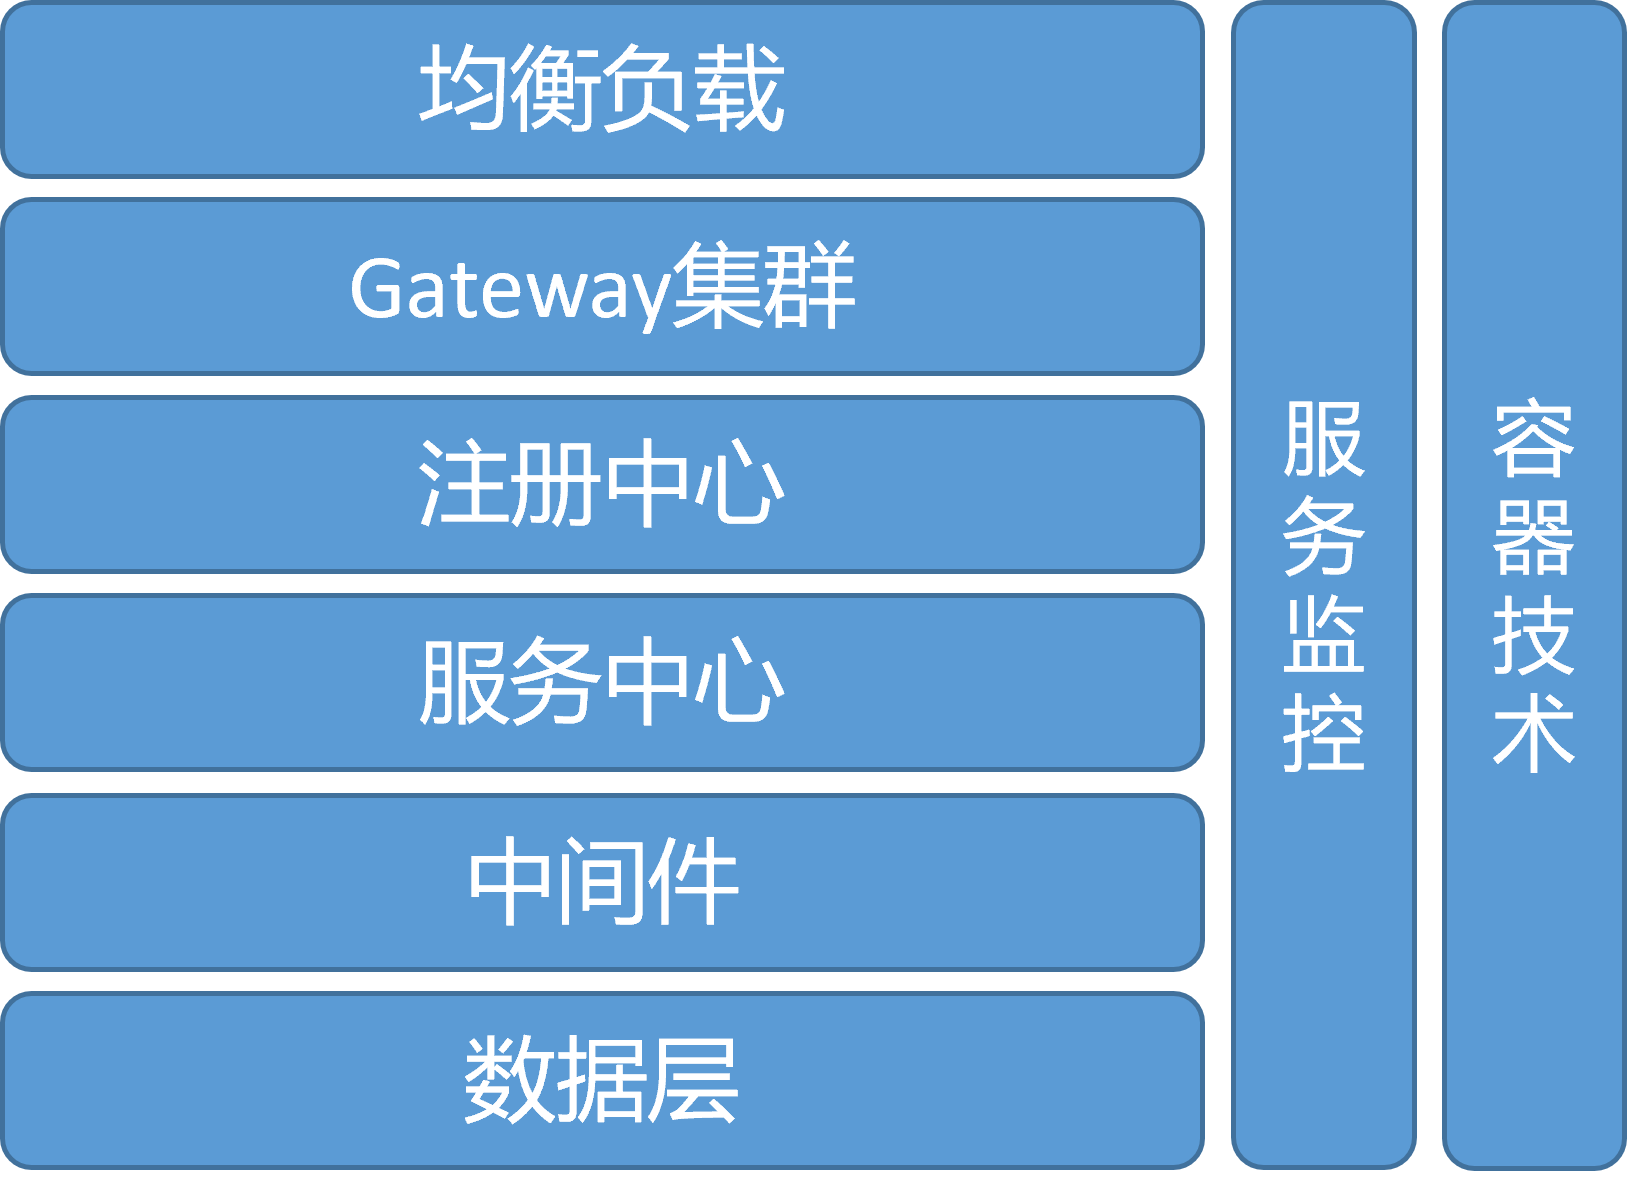
\includegraphics[scale=0.75]{figure/back_arch.png}
  \caption{\textbf{服务端架构图}}
  \label{fig:back_arch}
\end{figure}

\figref{fig:back_arch}是PhoeniX的服务端架构图,为了更好地解释该架构图,在此对下文中出现的一些专有名词进行解释:

\begin{enumerate}
  \item Kuberbetes:一个用于自动部署,扩展和管理容器化应用程序的开源系统,该系统是众多大型网站后台的首选基础设施之一。
  \item Prometheus:由SoundCloud开发的系统监控和预警工具,Prometheus也是开源软件,常用于实时监控虚拟容器的状态。
  \item LVS:Linux Virtual Server的缩写,通常用于均衡负载,将用户流量分发到不同的服务器上,重复利用服务端的资源。
  \item Etcd:提供分布式的键值对存储服务,通常用于微服务架构中的服务注册与发现,存储微服务的一些元信息。
  \item gRPC:开源高性能的RPC框架,用于各个微服务之间的相互调用,当用户的请求较为复杂时,可能需要几个微服务共同完成一个用户请求。
  \item RabbitMQ:一个消息队列,在生产者系统与消费者系统之间充当中间件,常用于对流量进行削峰,解决生产速率与消费速率不一致的问题。
\end{enumerate}

PhoeniX服务端以Golang作为主要编程语言,采用微服务架构,相比于传统的分层式架构,微服务架构能够承受更高的并发流量。我们采用Kubernetes作为服务端的运维基础,使用Prometheus对部署的各个服务进行监控。PhoeniX的服务端能够支撑高并发请求,用户流量到达服务端时,首先会到达LVS均衡负载层,均衡负载层会将请求分流到网关(Gateway)集群中的各个服务器。网关服务器提供聚合服务、路由等功能,流量经过网关服务器后到到Etcd注册中心,随后分发给对应的微服务。各个微服务采用Gin框架编写核心逻辑,使用gRPC作为RPC框架。服务中心请求数据时,将请求发送到消息中间件RabbitMQ中,不直接从MySQL等数据库中读取数据,起到流量削峰的作用。